\section{Motivation}
\label{sec:Motivation}

\begin{wrapfigure}{r}{0.43\textwidth}
		\vspace{-0.9cm}
		\centering
		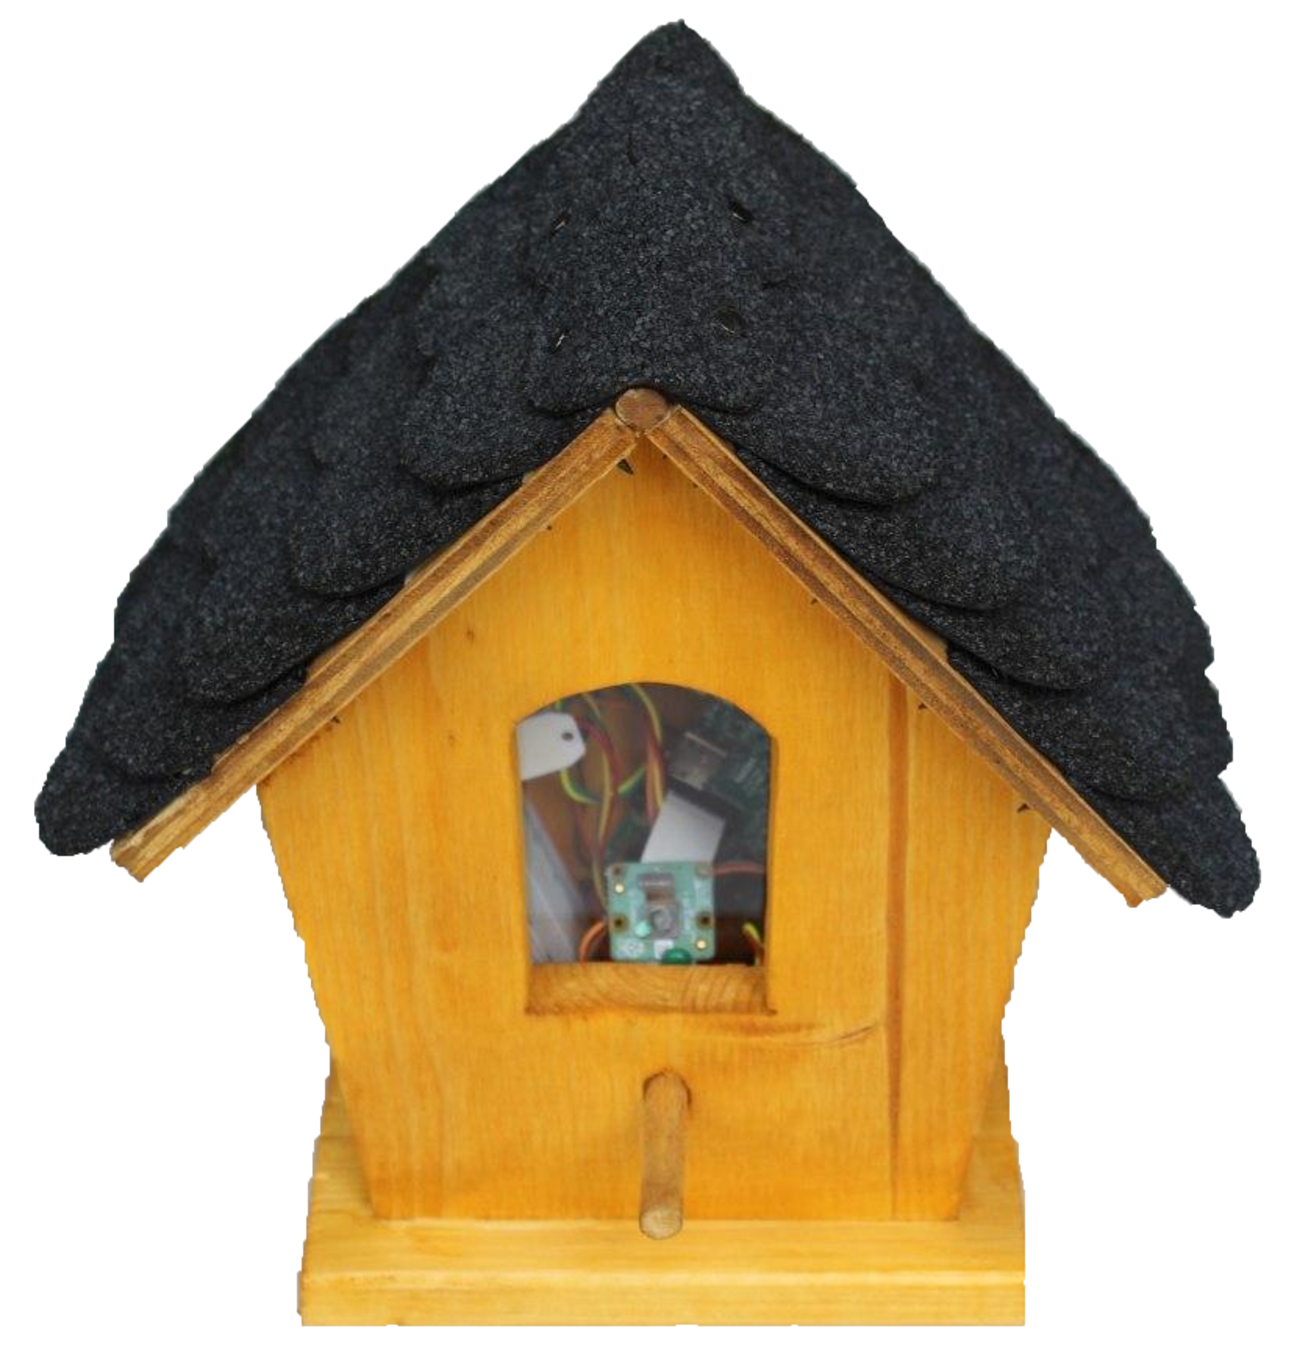
\includegraphics[width=0.4\textwidth]{./pictures/wetterstation.pdf}
		\caption{Wetterstation zur Aufnahme von Wetterdaten.}
		\label{fig:name}
		\vspace{-0.5cm}
\end{wrapfigure}
Das weatherpi Projekt entsteht im Rahmen des Physikstudiums.
Es widmet sich der Fragestellung, ob sich mit einfachen Mitteln zuverlässige
Wettervorhersagen erstellen lassen können.
Dazu werden lokale Wetterdaten mittels Sensoren, welche an einem 
Einplatinencomputer (Raspberry Pi) angeschlossen sind, erhoben.
Die aufgezeichneten Daten werden auf einen zentralen Server hochgeladen.
Ziel ist es, die lokalen Daten von mehreren Wetterstationen auszuwerten, um eine
flächendeckende Wetterprognose abzugeben. 

Zu den erhobenen Daten zählen die Temperatur, der Druck, die Luftfeuchtigkeit,
sowie ein Ausschnitt der Wolkendecke.
Inhalt dieses Papers ist die Wolkenklassifizierung, die ein Teil der
Wetteranalyse bildet.
Diese ist zur Spezifizierung der aktuellen Wetterlage notwendig.
Um Korrelationen zwischen den Attributen und der Bewölkung zu prüfen,
müssen die Daten bei bekannter Bewölkung aufgenommen werden.
Besteht eine Korrelation, so könnte in einem weiteren Schritt die Wolkendecke
als ein zusätzliches Attribut genutzt werden, um die anderen Wetterdaten genauer
vorherzusagen. 

Die erhobenen Wolkendaten sollen nach einem Training auf einem rechenstärkeren
Computer, mittels einer Live-Analyse auf dem Einplatinencomputer ausgewertet 
werden.
Die Auswertung steht unter der Prämisse schnell, genau und ressourcenschonend 
zu seien.
Dazu werden Algorithmen des maschinellen Lernenens verwendet, welche auf einen
klassifizierten Datensatz trainiert werden. 
Diese sollen bei hinreichend großer Genauigkeit die Klassenzugehörigkeit
automatisch erkennen.
Wenn das Klassenlabel bekannt ist, muss nicht mehr die gesamte Datenmenge des
Fotos zum Server geschickt werden und der Datentransfer kann reduziert werden. 
Desweiteren kann die Rechenlast auf die Rasperry Pis, welche in der Regel 
nicht ausgelastet sind, vom Server ausgelagert werden. 

Dazu werden zwei Modelle evaluiert, welche auf den charakteristischen
Eigenschaften des Wolkenspektrums trainiert werden. 
Diese sind einerseits die Formen und andererseits das Farbspektrum der Wolken.
Aus dem aufgenommenen Foto wird ein diskretes Farbspektrum erstellt, welches 
mit einem Random Forest ausgewertet werden kann.
Dabei bietet der Random Forest ein hohen Schutz gegen Übertraining.
Mittels eines Convolutional Neuronal Network (CNN) besteht die Möglichkeit, auf
dem Farbspektrum der Wolken sowie deren Formen zu trainieren. 
Die erhöhte Informationsdichte, mit der das CNN trainiert werden kann, 
lässt bei einem ausreichend generalisierten Training auf einen leistungs 
Schub gegenüber dem Random Forest schließen.

% Werden die Wolken entsprechend richtig klassifiziert laesst sich in weiteren
% Schritten welche nicht Teil dieses Papers sind aus der Folge der Wolken z.B
% der Niederschlag berechnen. 
% Desweiteren kann die entwicklung der Temperatur aufgrund der Waermespeicherung
% und Isolierug von Wolken verbessert werden.

